\documentclass{article}

\usepackage[left=1in, right=1in, top=1in, bottom=1in]{geometry}

\usepackage{setspace}
\usepackage{fancyhdr}
\usepackage{hyperref}
\usepackage{amsthm}
\usepackage{amssymb}
\usepackage{multirow}
\usepackage{enumitem}
\usepackage{graphicx}
\usepackage{makecell}
\usepackage{booktabs}
\usepackage{titlesec}
\usepackage{amsmath}
\usepackage{pdfpages}
\usepackage{enumitem}
\usepackage{caption}

\setcounter{secnumdepth}{4}

\hypersetup{
    colorlinks=true,     
    urlcolor=magenta
}

\renewcommand{\qedsymbol}{\rule{0.7em}{0.7em}}

\newlength\tindent
\setlength{\tindent}{\parindent}
\setlength{\parindent}{0pt}
\renewcommand{\indent}{\hspace*{\tindent}}
\setlength{\parskip}{0em}

\newenvironment{blockquote}{%
  \par%
  \vskip1em
  \leftskip=2em\rightskip=2em%
  \noindent\ignorespaces}{%
  \par\vskip1em}

\newenvironment{blockquote2}{%
	\par%
	\vskip1em
	\leftskip=4em\rightskip=4em%
	\noindent\ignorespaces}{%
	\par\vskip1em}

\pagestyle{fancy}
\fancyhf{}
\fancyhead[LO]{STA5176}
\fancyhead[RO]{Kyle Ligon}
\fancyfoot[LO]{Chapter 8 and 9}
\fancyfoot[RO]{\thepage}
 
\renewcommand{\headrulewidth}{0.5pt}
\renewcommand{\footrulewidth}{0.5pt}

\begin{document}
\section*{Chapter 8 and 9 Homework}
\subsection*{Due 3-18-2018}
\subsubsection*{Problem 9.13}
\subsubsection*{ a) Assess ANOVA assumptions using the graph from PROC MIXED.}

In order to proceed with ANOVA, we must check for the following pieces:
\begin{itemize}[leftmargin=+.5in]
 	\item[$\bullet$] No obvious pattern in our Residual Scatterplot
	\item[$\bullet$] Normal shape to the Residual Histogram.
 	\item[$\bullet$] Residuals fit along the linear prediction of our Actual "Normality" to the Theoretical Normal Model.  
\end{itemize}

Since there is no readily observable pattern in our residuals, our distribution is mound shaped, and our Residuals fit the along the Q-Q plot(although, there may be evidence of a right skew), we will proceed with ANOVA to see if at least one mean is different.  

\begin{figure}[h]
\centering
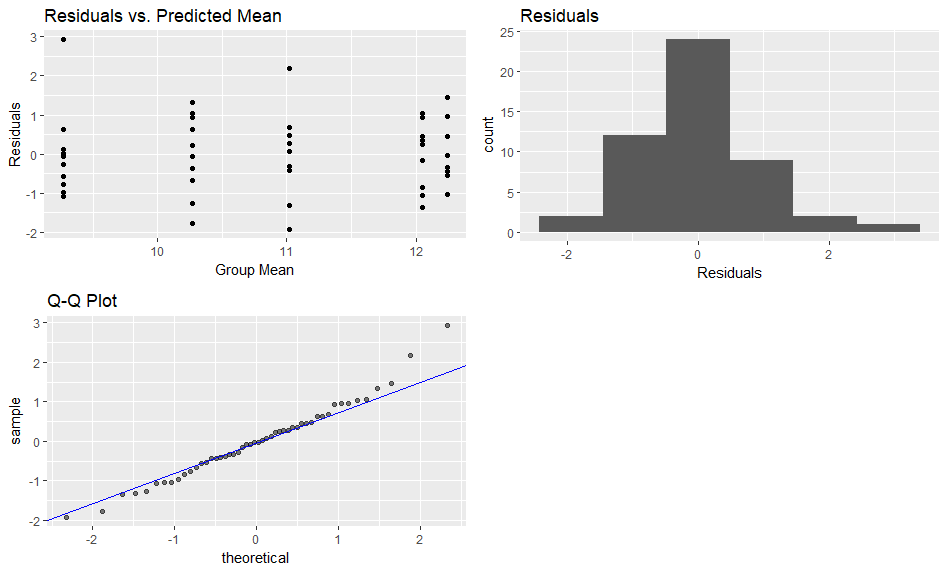
\includegraphics[width = 1.0\textwidth]{AnovaCheck.png}
\end{figure}

\pagebreak

\subsubsection*{ b) Perform ANOVA to determine if there is a difference among the five weight-reducing agents, $\alpha$ = 0.05.} 
\begin{table}[ht]
\caption{ANOVA Table for Weight Loss Study}
\centering
\begin{tabular}{l c c c c c}
\hline\hline
Row Names & SS & df & MS & F & P-Value \\ [0.5ex] 
\hline
Treatments (T) & 61.618 & 4 & 15.4045 & 15.6805 & 4.16x$10^{-8}$ \\
Error (E) & 44.207 & 45 & 0.9824 & \\
Total & 105.825 & 49 &  \\ [1ex]
\hline
\end{tabular}
\label{table:nonlin}
\end{table}

Hypotheses:
\begin{blockquote}
$H_{0}$: $\mu_{a1}$ = $\mu_{a2}$ = $\mu_{a3}$ = $\mu_{a4}$ = $\mu_{s}$ \\
$H_{1}$: At least one mean is different.  
\end{blockquote}
Test Statistic:
\begin{blockquote}
F = 15.6805
\end{blockquote}
Rejection Region:
\begin{blockquote}
Reject $H_{0}$ if $F_{0} > F_{\alpha, 4, 45}$ \\
$F_{0.95, 4 , 45} = 5.72$
\end{blockquote}
Conclusion/Interpretation:
\begin{blockquote}
Since our $F_{0} > 5.72$, there is strong enough evidence to support rejecting the null hypothesis that the means are the same.  The data provided does suggest at least one mean is different from the rest.  
\end{blockquote}


\subsubsection*{ c) Determine significantly different pairs using Tukey's W with $\alpha$ = 0.05}
\begin{blockquote}
To find which groups are different from each other, we will utilize Tukey's W to check which means are different from one another.  We will verify this by checking which one's p-values are less than 0.05 after using the TukeyHSD test on our ANOVA Model in R.  
\end{blockquote}
Conclusion/Interpretation
\begin{blockquote}
With our Tukey W test being run, the differences lie in the following means:
\end{blockquote}

\begin{itemize}[leftmargin=+0.5in]
	\item[$\bullet$] S differs with $A_{1}$, $A_{2}$, and $A_{4}$
	\item[$\bullet$] $A_{3}$ differs with $A_{1}$ and $A_{4}$
\end{itemize}

\pagebreak

\subsubsection*{ d) Determine which, if any, of the new agents have significantly larger mean weight loss as compared to the standard agent; $\alpha$ = 0.05}

\begin{blockquote} 
Using s as our control, we will performs Dunnett's test to determine if there's a significantly larger difference with the new agents.  The first step in checking out if any of the new agents are yielding better weight loss results is to find Dunnett's D.  
\end{blockquote}

\begin{eqnarray}
D = d_{\alpha}(k,v)\sqrt{\frac{2s^{2}_{W}}{n}} \nonumber \\ 
D = d_{0.05}(4,45)\sqrt{\frac{2(0.982)}{10}} \nonumber \\
D = 2.23\sqrt{\frac{1.964}{10}} \nonumber \\
D = 2.23(0.4432) \nonumber \\
D = 0.9888 \nonumber
\end{eqnarray}

\begin{table}[h]
\caption{Dunnett's Control Test}
\centering
\begin{tabular}{c c c c}
\hline\hline
Treatment & $\bar{y}_{i}-\bar{y}_{c}$ & Comparison & Conclusion \\ [0.5ex] 
\hline
a1 & 2.78 & $>$ D & Greater Than Control \\
a2 & 1.75 & $>$ D & Greater Than Control \\
a3 & 1.00 & $>$ D & Greater Than Control \\ 
a4 & 2.97 & $>$ D & Greater Than Control \\ [1ex]
\hline
\end{tabular}
\label{table:nonlin}
\end{table}    

Conclusion/Interpretation:
\begin{blockquote}
All four of the agents are statistically significant. Thus, we can reject the null hypotheses that the difference in weight loss metrics between the original agent(s) and the new agents($a_{1}, a_{2}, a_{3},$ and $a_{4}$) is zero.  Each of the new agents appear to have an increase in weight loss over the agent s.    
\end{blockquote}

\subsubsection*{9.17 - construct the contrasts}





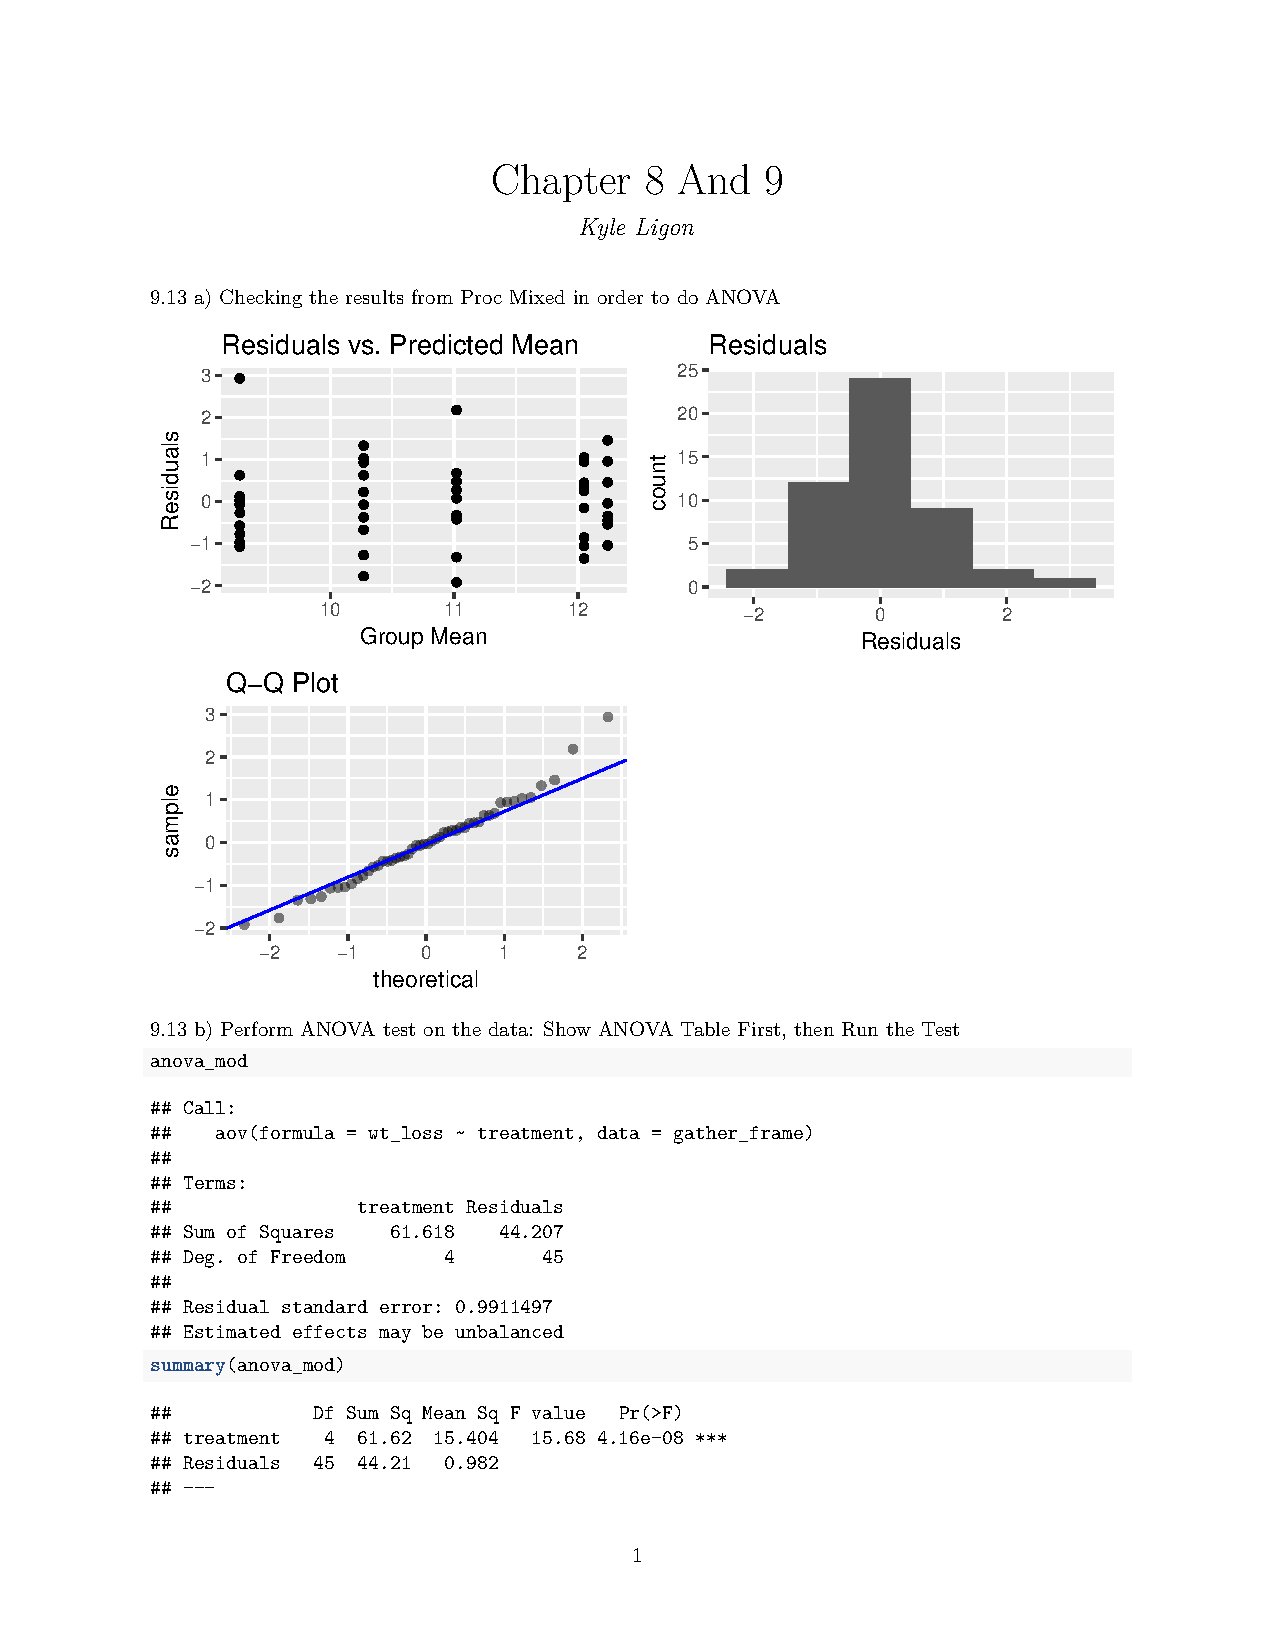
\includepdf[pages=-]{Chapter_8_And_9.pdf}
\end{document}



